\documentclass{../exam-zh}
\usepackage{siunitx}

\examsetup{
  page/size=a4paper,
  paren/show-paren=true,
  paren/show-answer=true,                   % 教师版：显示选择题答案
  fillin/show-answer=true,                  % 教师版：显示填空题答案
  solution/show-solution=show-move,         % 教师版：在末尾生成解答
  solution/label-indentation=false          % 教师版：解答无缩进
}

\everymath{\displaystyle}

\title{2028届高一第二学期数学限时作业（10）教师用卷}
% \subject{数学（理科）}


\ExamPrintAnswerSet[
  % —— 可选参数：覆盖命令 ——
  \title{2028届高一第二学期数学限时作业（10）}
  % \subject{数学（理科）}
  \RenewDocumentCommand \warning { O{} m } {},
  \RenewDocumentEnvironment { notice } { O{} O{} +b } {} {}
]{
  % —— 必选参数：覆盖键值 ——
  paren/show-answer=false,                 % 学生版：不显示选择题答案
  fillin/show-answer=false,                % 学生版：不显示填空题答案
  solution/show-solution=hide,             % 学生版：不生成解答
}

\begin{document}

\maketitle

\information{
  学校\underline{\hspace{6em}},
  姓名\underline{\hspace{6em}},
  班级\underline{\hspace{6em}},
  考号\underline{\hspace{6em}}
}
% \warning{（在此卷上答题无效）}

本试卷共 4 页，22 题。全卷满分 150 分。考试用时 120 分钟。


% \begin{notice}
%   \item 答卷前，考生务必将自己的姓名、考生号、考场号和座位号填写答题卡上，用2B铅笔将试卷类型（B）填涂在答题卡相应位置上，将条形码横贴在答题卡右上角“条形码粘贴处”。
%   \item 作答选择题时，选出每小题答案后，用2B铅笔在答题卡上对应题目选项的答案信息点涂黑；如需改动，用橡皮擦干净后，再选涂其他答案。答案不能答在试卷上。
%     写在试卷、草稿纸和答题卡上的非答题区域均无效。
%   \item 非选择题必须用黑色字迹的钢笔或签字笔作答，答案必须写在答题卡各题目指定区域内相应位置上；如需改动，先划掉原来的答案，然后再写上新答案；不准使用铅笔和涂改液。不按以上要求作答无效。
%   \item 考生必须保持答题卡的整洁。考试结束后，将试卷和答题卡一并交回。
% \end{notice}

\section{%
  单选题：本题共 8 小题，每小题 5 分，共 40 分。
  在每小题给出的四个选项中，只有一项是符合题目要求的。
}

% 1.
\begin{question}
  已知 $\vec{a}=(2,4)$, $\vec{b}=(1,t)$, 若 $(\vec{a}+\vec{b})\parallel(\vec{a}-3\vec{b})$, 则实数 $t=$ \paren[D]

  \begin{choices}
    \item $-2$
    \item $\frac{1}{2}$
    \item $1$
    \item $2$
  \end{choices}

  \begin{solution}
    D.

    因为$\vec{a}=(2,4)$, $\vec{b}=(1,t)$, 所以$\vec{a} + \vec{b} = (3, 4+t), 3\vec{a} - \vec{b} = (5, 12-t)$. 由$(\vec{a} + \vec{b})\parallel(3\vec{a} - \vec{b})$ 可知$3(12-t) - 5(4+t) = 0$, 解得$t = 2$.
  \end{solution}
\end{question}

% 2.
\begin{question}
  设 $m,n$ 是两条不同的直线, $\alpha,\beta$ 是两个不同的平面, 则下列结论正确的是 \paren[D]
  \begin{choices}
    \item 若 $m\parallel\alpha$, $n\parallel\alpha$, 则 $m\parallel n$
    \item 若 $m\parallel n$, $m\parallel\alpha$, 则 $n\parallel\alpha$
    \item 若 $m\subset\alpha$, $n\subset\beta$, 则 $m,n$ 是异面直线
    \item 若 $\alpha\parallel\beta$, $m\subset\alpha$, $n\subset\beta$, 则 $m\parallel n$ 或 $m,n$ 是异面直线
  \end{choices}

  \begin{solution}
    D.
    \begin{itemize}
      \item 对于$A$, 若$m\parallel\alpha, n\parallel\alpha$, 则$m, n$平行或相交或为异面直线, 故$A$错误.
      \item 对于$B$, 若$m\parallel n, m\parallel\alpha$, 则$n\parallel\alpha$或$n\subset\alpha$, 故$B$错误.
      \item 对于$C$, 若$m\subset\alpha, n\subset\beta$, 当平面$\alpha, \beta$相交时, $m, n$可能相交, 故$C$错误.
      \item 对于$D$, 若$\alpha\parallel\beta$, $m\subset\alpha$, $n\subset\beta$, 则$m, n$无公共交点, 故$m, n$平行或为异面直线, 故$D$正确.
    \end{itemize}
  \end{solution}
\end{question}

% 3.
\begin{question}
  下列关于空间几何体的论述, 正确的是 \paren[D]
  \begin{choices}
    \item 有两个面平行, 其他各个面都是平行四边形的多面体是棱柱.
    \item 有两个平面平行且相似, 其他各个面都是梯形的多面体是棱台.
    \item 连接圆柱上下底面圆周上任意两点的线段是圆柱的母线.
    \item 圆台的轴截面不可能为直角梯形.
  \end{choices}
\end{question}

% 4.
\textfigure[fig-pos=right, text-width = 0.7\linewidth]{
  \begin{question}
    如图, 按斜二测画法所得水平放置的平面四边形 $ABCD$ 的直观图为梯形 $A'B'C'D'$．其中 $A'B'\parallel C'D'$, $A'B'\perp B'C'$, $A'B'=4$, $D'C'=1$．以原四边形 $ABCD$ 的边 $AD$ 为轴, 旋转一周得到的几何体体积为 \paren[C]
    \begin{choices}
      \item $62\pi$
      \item $21\sqrt{2}\pi$
      \item $42\sqrt{2}\pi$
      \item $63\sqrt{2}\pi$
    \end{choices}
  \end{question}
}{
  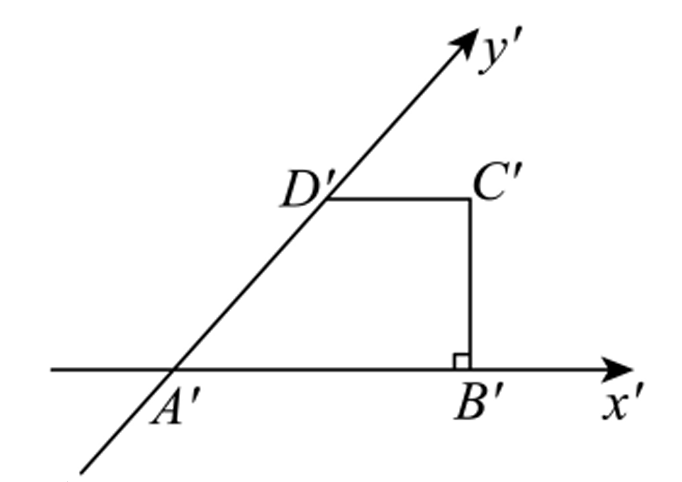
\includegraphics[width=0.3\linewidth]{figure/4.png}
}

% 5.
\begin{question}
  已知向量 $\vec{e}_1$, $\vec{e}_2$ 非零, 则 “$|\vec{e}_1+\vec{e}_2|=|\vec{e}_1|+|\vec{e}_2|$” 是 “存在非零实数 $m$, $n$, 使得 $m\vec{e}_1+n\vec{e}_2=0$” 的 \paren[A]
  \begin{choices}
    \item 充分不必要条件.
    \item 必要不充分条件.
    \item 充要条件.
    \item 既不充分也不必要条件.
  \end{choices}
\end{question}

% 6.
\begin{question}
  $D$ 是 $\mathrm{Rt}\triangle ABC$ 斜边 $BC$ 上一点, 若 $AB=AD$, $AC=\sqrt{3}DC$, 则 $\sin\angle ABC = $ \paren[D]
  \begin{choices}
    \item $\dfrac{1}{2}$
    \item $\dfrac{\sqrt{3}}{3}$
    \item $\dfrac{\sqrt{2}}{2}$
    \item $\dfrac{\sqrt{3}}{2}$
  \end{choices}
\end{question}

% 7.
\textfigure[fig-pos=right, text-width = 0.7\linewidth]{
  \begin{question}
    如图所示, 在边长为$4$的正八边形$ABCDEFGH$中, 点$O$是正八边形的中心, 点$P$是其内部任意一点. 则$\overrightarrow{OA}\cdot\overrightarrow{PA} + \overrightarrow{OF}\cdot\overrightarrow{PA}$的取值范围是 \paren[A]
    \begin{choices}
      \item $(-8\sqrt{2}, 16+8\sqrt{2})$.
      \item $(-16, 16+8\sqrt{2})$.
      \item $(-8, 16)$.
      \item $(-16, 16)$.
    \end{choices}
  \end{question}
  }{
  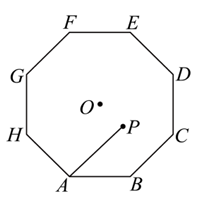
\includegraphics[width=0.3\linewidth]{figure/7.png}
}

% 8.
\begin{question}
  已知平行六面体$ABCD-A_1B_1C_1D_1$的所有棱长均为$2$, $O$为$AC$的中点, 且$A_1O\perp$平面$ABCD$, 若直线$AA_1$与底面$ABCD$的夹角为$45^\circ$, 则三棱锥$A-A_1BD$的外接球被平面$BCC_1B$截得的截面面积为 \paren[C]
  \begin{choices}
    \item $\frac{2\pi}{3}$.
    \item $\pi$.
    \item $\frac{4\pi}{3}$.
    \item $2\pi$.
  \end{choices}
\end{question}

\section{%
  多选题：本题共 3 小题，每小题 5 分，共 15 分。
  在每小题给出的选项中，有多项符合题目要求。
  全部选对的得 5 分，部分选对的得 2 分，有选错的得 0 分。
}

% 9.
\textfigure[fig-pos=right, text-width = 0.7\linewidth]{
  \begin{question}
    如图, 在平行四边形 $ABCD$ 中, $E$ 为 $CD$ 的中点, $\overrightarrow{AF}=\dfrac{1}{3}\overrightarrow{AE}$, 则 \paren[BCD]
    \begin{choices}
      \item $\overrightarrow{AE}=\overrightarrow{BC}-\dfrac{1}{3}\overrightarrow{BA}$.
      \item $\overrightarrow{BE}=\overrightarrow{BC}+\dfrac{1}{2}\overrightarrow{BA}$.
      \item $\overrightarrow{BF}=\dfrac{1}{3}\overrightarrow{BC}+\dfrac{5}{6}\overrightarrow{BA}$.
      \item $\overrightarrow{AE}+\overrightarrow{BE}=2\overrightarrow{BC}$.
    \end{choices}
  \end{question}
}{
  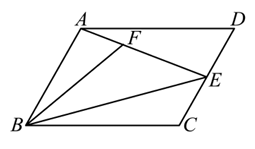
\includegraphics[width=0.3\linewidth]{figure/9.png}
}

% 10.
\begin{question}
  已知 $\triangle ABC$ 三个内角 $A,B,C$ 对边分别是 $a,b,c$, 若 $(\sqrt{3}c - 2a\sin B)\sin C = \sqrt{3}(b\sin B-a\sin A)$, 则下列选项正确的是 \paren[BCD]
  \begin{choices}
    \item $B=\dfrac{\pi}{6}$.
    \item 若 $D$ 是 $AC$ 边上的一点, 且 $\overrightarrow{CD}=2\overrightarrow{DA}$, $BD=2$, 则 $\triangle ABC$ 的面积的最大值为 $\dfrac{3\sqrt{3}}{2}$.
    \item 若 $\triangle ABC$ 是锐角三角形, 则 $\dfrac{c}{a}$ 的取值范围是 $\left(\dfrac{1}{2},2\right)$.
    \item 若 $O$ 是 $\triangle ABC$ 的外心, $\overrightarrow{OB}=m\overrightarrow{OA}+n\overrightarrow{OC}$, 则 $m+n\in[-2,1)$.
  \end{choices}
\end{question}

% 11.
\textfigure[fig-pos=right, text-width = 0.7\linewidth]{
  \begin{question}
    如图, 在矩形$ABCD$中, $AD=2AB=4$, $E$为$BC$的中点. 将$\triangle BAE$沿$AE$向上翻折到$\triangle PAE$, 连接$PC, PD$, 在翻折过程中, 下列说法正确的是 \paren[AD]
    \begin{choices}
      \item 若平面$PAE\perp$平面$ABCD$, 则$PA\perp DE$.
      \item 四棱锥$P-AECD$的体积最大值为$4\sqrt{2}$.
      \item 点$P$从点$B$翻折到$AD$中点的过程中, $PD$的中点$F$形成的轨迹长度为$\sqrt{2}\pi$.
      \item 三棱锥$P-AED$的外接球表面积的最小值为$16\pi$.
    \end{choices}
  \end{question}
}{
  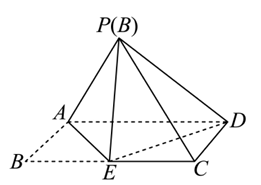
\includegraphics[width=0.3\linewidth]{figure/11.png}
}
\section{填空题：本题共 3 小题，每小题 5 分，共 15 分。}

% 12.
\begin{question}
  已知 $\vec{a}=(2,3)$, $\vec{b}=(-1,0)$, 则 $\vec{a}$ 在 $\vec{b}$ 方向上的投影向量为 \fillin[$(2, 0)$]（用坐标表示）.
  \begin{solution}
    \textbf{以下均为占位符}
    由 $f(x) = f(-x)$，得 $a = 1$。
  \end{solution}
\end{question}

% 13.
\begin{question}
  在棱长为 $4$ 的正方体 $ABCD-A_1B_1C_1D_1$ 中, 点 $C$ 到平面 $C_1BD$ 的距离为 \fillin[$\frac{4\sqrt{3}}{3}$].
\end{question}

% 14.
\begin{question}
  已知某正三棱锥的底面边长为 $4$, 侧面与底面所成二面角的余弦值为 $\dfrac{2}{3}$, 球 $O_1$ 为该三棱锥的内切球．球 $O_2$ 与球 $O_1$ 相切, 且与该三棱锥的三个侧面也相切, 则球 $O_2$ 与球 $O_1$ 的表面积之比为 \fillin[$\frac{1}{25}$].
\end{question}
\section{解答题：本题共 5 小题，共 70 分。解答应写出文字说明、证明过程或演算步骤。}

% 15.
\begin{problem}[points = 10]
  四棱台的上下底面边长分别为 $2$ 和 $4$, 侧棱长为 $4$.
  \begin{enumerate}
    \item 求它的表面积;
    \item 求它的体积.
  \end{enumerate}
\end{problem}

% 16.
\begin{problem}[points = 12]
  已知向量 $\overrightarrow{OA}=(1,1)$, $\overrightarrow{OB}=(3,-1)$, $\overrightarrow{OC}=(m,3)$, $\overrightarrow{OD}=(x,y)$, 其中 $O$ 为坐标原点．
  \begin{enumerate}
    \item 若 $A,B,C$ 三点共线, 求实数 $m$ 的值;
    \item 当四边形 $ABCD$ 为矩形时, 设点 $M$ 为线段 $CD$ 的中点, 问在线段 $AD$ 上是否存在点 $N$ 使得 $|\overrightarrow{NB}+\overrightarrow{NM}|=\dfrac{\sqrt{194}}{3}$, 若存在, 请求出所有满足条件的点 $N$ 的坐标, 若不存在, 说明理由．
  \end{enumerate}
\end{problem}

% 17.
\textfigure[fig-pos=bottom-flushright]{
  \begin{problem}[points = 12]
    “我将来要当一名麦田里的守望者, 有那么一群孩子在一块麦田里玩, 几千万的小孩子, 附近没有一个大人,我是说……除了我”《麦田里的守望者》中的主人公霍尔顿将自己的精神生活寄托于那广阔无垠的麦田. 假设霍尔顿在一块成凸四边形$ABCD$的麦田里成为守望者. 如图所示,为了分割麦田, 他将$BD$连接, 设$\triangle ABD$中边$BD$所对的角为$A$, $\triangle BCD$中边BD所对的角为$C$. 经测量知$AB = BC = CD = 2, AD = 2\sqrt{3}$.
    \begin{enumerate}
      \item 若$A = 30^\circ$, 求$C$;
      \item 霍尔顿发现无论$BD$多长, $\sqrt{3}\cos A - \cos C$为一个定值. 请你验证霍尔顿的结论, 并求出这个定值.
      \item 霍尔顿发现麦田的的生长与土地面积的平方呈正相关, 记$\triangle ABD$与$\triangle BCD$ 的面积分别为$S_1$和$S_2$, 为了更好地规划麦田, 请你帮助霍尔顿求出$S_1^2 + S_2^2$的最大值.
    \end{enumerate}
  \end{problem}
}{
  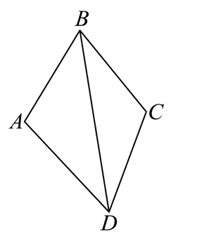
\includegraphics[width=3cm]{figure/17.png}
}

% 18.
\begin{problem}[points = 12]
  \textfigure[fig-pos=bottom-center]{
    矩形$ABCD$中, $AB = 2AD = 2$, $P$为线段$DC$的中点. 将$\triangle ADP$沿着$AP$折起, 使得平面$ADP\perp$平面$ABCP$. 在新构造的四棱锥$D-PABC$中, 求解以下问题:
    \begin{enumerate}
      \item 求四棱锥$D-PABC$的体积.
      \item 求二面角$P-AD-B$的余弦值.
      \item 在$DC$上是否存在点$E$使得$AD\parallel$平面$PBE$? 若存在, 求出点$E$的位置; 若不存在, 请说明理由.
    \end{enumerate}
  }{
    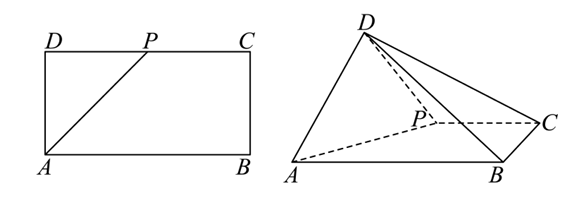
\includegraphics[width = 12cm]{figure/18.png}
  }
\end{problem}

% 19.
\begin{problem}[points = 12]
  已知$s$是直线$PQ$外一点, 点$M, N$在直线$PQ$上.（点$M, N$与点$P, Q$任一点均不重合）我们称如下操作为“由$s$点对$PQ$施以视角运算”:
  \begin{itemize}
    \item 若点$M$在线段$PQ$上, 记$(P, Q; M) = \frac{\left|SP\right|\sin\angle PSM}{\left|SQ\right|\sin\angle MSQ}$; 
    \item 若点$M$在线段$PQ$外, 记$(P, Q; M) = -\frac{\left|SP\right|\sin\angle PSM}{\left|SQ\right|\sin\angle MSQ}$.
  \end{itemize}
  并且记$(P, Q; M, N) = \frac{(P, Q; M)}{(P, Q; N)}$. 记$\triangle ABC$的内角$A, B, C$的对边分别为$a, b, c$. 已知$b=2$, $A = 60^\circ$, $D$是射线$BC$上的一点. 现由$A$点对$BC$施以视角运算, 得到$(B, C; D) = \frac{c}{2}$.
  \begin{enumerate}
    \item 若$\left|AD\right| = \sqrt{3} + 1$, 求$\overrightarrow{AD}\cdot\overrightarrow{DC}$的值;
    \item 射线$BC$上的点$M$满足$(B, C; M, D) = -2$.
    \begin{enumerate}
      \item 求$\angle CAM$;
      \item 求$\left|AM\right| + 16\left|AD\right|$的最小值.
    \end{enumerate}
  \end{enumerate}

  \begin{solution}
    函数的定义域为 $(0, +\infty)$,
    又 \[f^{\prime}(x) = 1 - \ln x-1 = -\ln x, \score{2}\]
    当 $x \in(0, 1)$ 时, $f^{\prime}(x) > 0$, 当 $x \in(1, +\infty)$ 时, $f^{\prime}(x) < 0$,
    故 $f(x)$ 的递增区间为 $(0,1)$, 递减区间为 $(1, +\infty)$.
  \end{solution}
\end{problem}


\end{document}
